\titleformat{\chapter}[display]{\normalfont\LARGE\bfseries}{}{1em}{\thechapter.~}

\chapter{Laboratorio:  Programación de Autómatas Lógicos}


\section{Objetivos}
Este  laboratorio busca:
\begin{itemize}
	{\small
    \item Entender la implementación de la norma IEC 61131-3.
    \item Programar  de manera estructura el PLC S7-1500 usando bloques OB, FB y DB.
    \item Utilizar tres lenguajes estandarizados para la programación de bloques lógicos.
    \item Solucionar problemas comunes de automatización.
 }
\end{itemize} 

 
\section{Equipos y materiales}
Para este laboratorio de necesitaran:
\begin{itemize}
	{\small 
	\item 1 PLC SIEMENS 1500.
	\item 1 Software TIA Portal V17.
	\item 1 Computadora.
	\item 1 \href{https://support.industry.siemens.com/dl/files/056/109815056/att_1121729/v4/STEP_7_WinCC_V18_esES_es-ES.pdf}{Manual del software TIA Portal}.
	\item 1 \href{https://cache.industry.siemens.com/dl/files/384/86140384/att_1131259/v1/s71500_et200mp_manual_collection_es-ES.pdf}{Colección de Manuales S7-1500}
}
\end{itemize}

\section{Marco de referencia}

La programación de los autómatas programables ha sufrido cambios en la semántica y sintaxis de programación con la implementacion de la norma IEC 611131-3 \cite{IEC61131-1} por parte de los fabricantes. La normalización de la semántica  mediante la estructuración de los programas y la normalización de sintaxis mediante la implementacion de cinco lenguajes de programación estandarizados  permiten la portabilidad del código entre fabricantes. 

La programación  estructura de  código informático para autómatas programables, permite organizar y descomponer  las soluciones en multiples subsistemas con distintos niveles de jerarquía. Esta  nueva forma de programar estructuradamente permite ordenar y dar mantenimiento al código de forma más sencilla, así como re-utilizar  código existente para otras soluciones. Al respecto la norma IEC-61131-3 \cite{Tiegelkamp10} indica que los autómatas modernos estructuran sus programas en \textit{Program Organisation Units} (POU) los cuales los divide en tres tipos: \textit{Program}, \textit{Function Block} y \textit{Funtion}.  

SIEMENS indica en su manual de Software \cite{TIA-S7}, que el programa de usuario se conforma por: bloques  de organización (OB), bloques de función (FB), funciones (FC), y bloques de datos (DB), la Figura \ref{fig:plc} muestra la relación entre los distintos bloques. Por favor leer entre las páginas 5625-5631 para una descripción detallada de los bloques.

\begin{figure}[H]
	\centering
	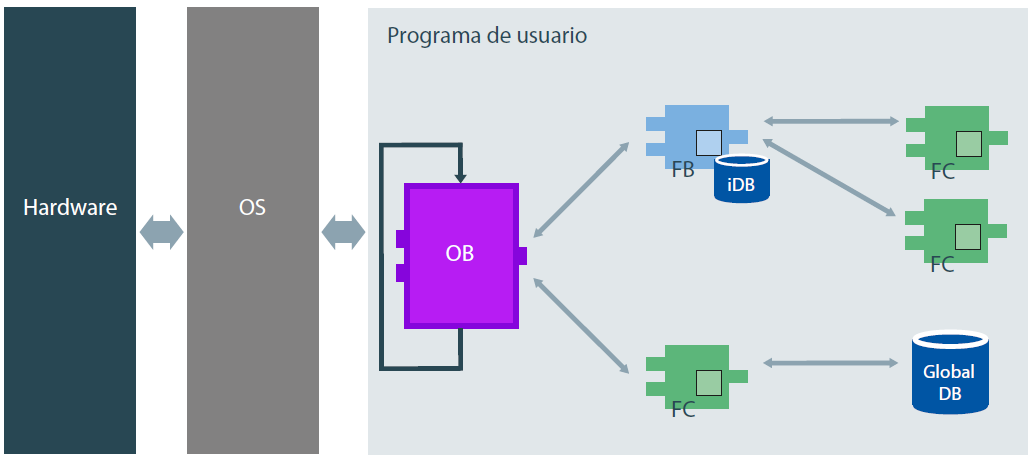
\includegraphics[width=0.85\linewidth]{Imagenes/PLC}
	\caption{Programación jerarquizadas en TIA Portal. }
	\label{fig:plc}
\end{figure}


Cada bloque OB, FB o FC puede ser programado con varios lenguajes estandarizados, es decir un FB puede ser programado de cinco formas distintas y también es permitido mesclar distintos lenguajes en la solución jerarquizada. La Figura \ref{fig:languajes} muestra los cinco lenguajes estandarizados por la norma: Diagrama en escalera (LD), Diagrama en Bloque de Funciones (FBD), Lista de Instrucciones (IL), Texto estructurado (ST) y Gráfico de Función Secuencial (SFC). Notese en la Figura \ref{fig:languajes}, que los primeros cuatro lenguajes muestran la respectiva implementación de una AND lógica entre las señales booleanas  S1  y S2. Al respecto SIEMENS nombra dichos lenguajes como: KOP o esquemas de contactos, FUP o diagrama de funciones, AWL o lista de instrucciones, SCL o lenguaje de control estructurado y GRAPH o lenguaje de programación gráfico. La descripción de detallada de cada lenguaje, sus funciones, ejemplos, etc., se encuentran en el manual del sistema \cite{TIA-S7}, para la funcionalidad del KOP incie en página 14161, para el FUP ver página 14223, para  AWL inicia en la página 14283, el SCL se encuentra en la página 14333 y para el GRAPH ver la página 14411.

\begin{figure}
	\centering
	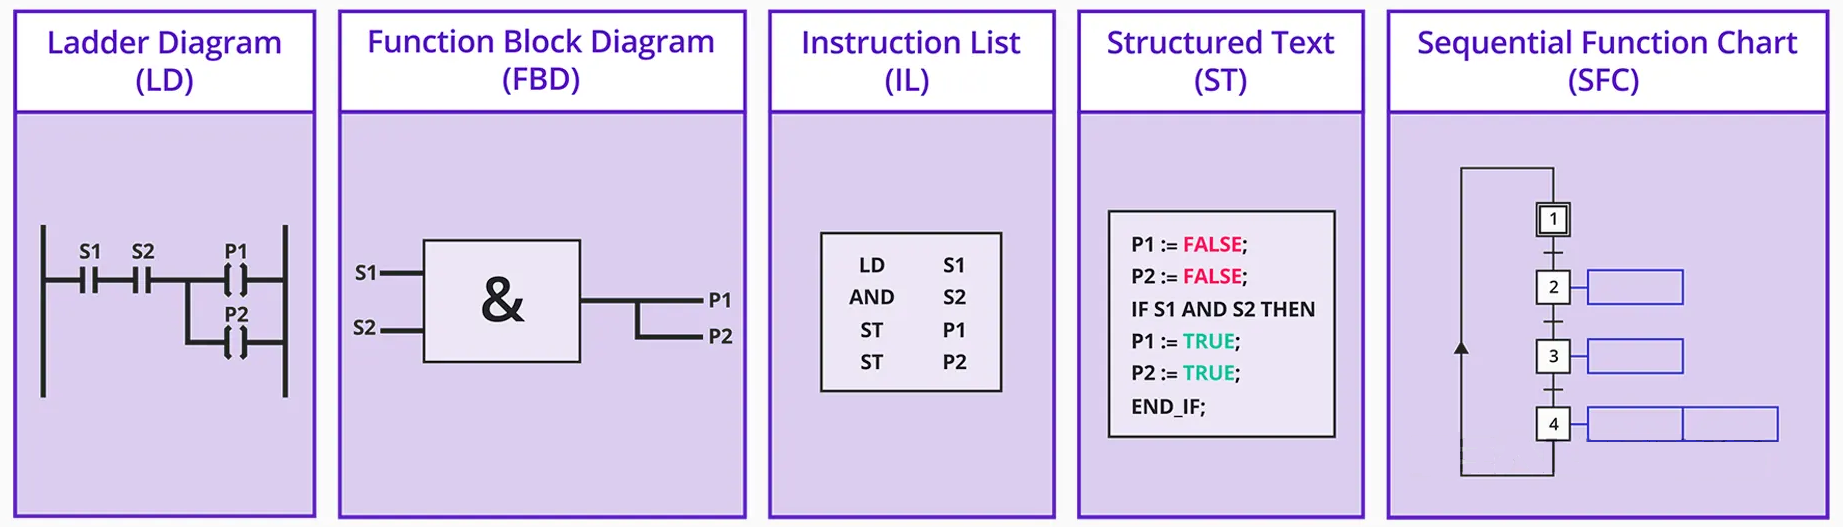
\includegraphics[width=1\linewidth]{Imagenes/Languajes}
	\caption{Lenguajes estandarizados por la norma IEC 61131-3.}
	\label{fig:languajes}
\end{figure}


Los diagramas electricos de conexión del CPU S7-1500, de sus módulos de entrada y salida se muestran en el manual del hardware \cite{PLC-1500}. La creación de un proyecto con el Software TIA portal se encuentra en la página  1280 de dicho manual, sin embargo, un video informativo con dicho procedimiento esta disponible en \cite{Maria}. 



 
\section{Metodología}

Este laboratorio tiene una duración de 4 lecciones, repartidas en dos semanas. Los estudiantes deben mostrar durante las clases programadas las tres actividades propuestas. Deben recabar fotografías y resultados de los equipos de medición para elaborar las evidencias. Las evidencias se subirán al TecDigital la semana siguiente finalizadas las actividades.

\section{Práctica en Clase}

\subsection{Actividad 1}

	Se requiere programar un arranque estrella-delta con multiples instancias. Para realizar esta actividad, utilize el lenguaje de contactos (KOP) para programar un  estrella - delta  dentro de un Bloque de función (FB). El FB tendrá como parámetros de entrada: la señal de arranque, pare, sobre carga y tiempo del temporizador. Como señales de salida tendrá la de la bobina general, la bobina que realiza el estrella y la bobina en delta.
	
	Luego en el bloque de organizacion uno (OB1), se llama el bloque  FB multiple veces. Por ejemplo, llame el FB tres veces y ponga tiempos de arranque distintos \{3, 6, 9\} segundos al parámetro tiempo  de  cada instancia.
	
 \subsubsection{Conteste las preguntas}
  
  Si se presiona el arranque al mismo tiempo, ¿como fue diagrama de tiempos de las 9 señales?
  ¿Puede mostrar el diagrama KOP del FB y OB1 implementado?
  

\subsection{Actividad 2}

Se necesita automatizar un parque de pozos profundos, el parque posee tres pozos y y tres tanques de captación. Se desea un sistema general que inicialice y pares los tres subsistemas, es decir, cuando se presione el arranque inicien el sistema de los tres pozos y cuando se presione el pare se detengan. Cuando se active una sobrecarga de algún motor ese subsistema en específico deja de funcionar, pero los otros dos subsistemas de pozos y tanque siguen funcionando normalmente. Los subsistemas se llamarán S1, S2 y S3 respectivamente.

Cada subsistema de pozo profundo se compone de dos bombas que funcionan en alternancia, un pozo de captación y un tanque de almacenamiento. Las señales del tanque de almacenamiento indican el nivel alto \textbf{T1-Na}, y nivel bajo \textbf{T1-Nb} de agua, el pozo profundo posee también dos sensores de nivel, nivel alto \textbf{P1-Na} y nivel bajo \textbf{P1-Nb}, además existen las dos señales de salida para las dos bombas: \textbf{S1-B1} y \textbf{S1-B2}. 

EL funcionamiento del subsistema es de la siguiente forma: las bombas toman el agua del pozo y la deposita en el tanque de captación. El nivel de agua \textbf{T1-Nb} activa la bomba \textbf{S1-B1} siempre y cuando la señal de \textbf{P1-Na} este activa. La bomba \textbf{S1-B1}  se apaga hasta alcanzar el nivel \textbf{T1-Na}  o que se quede sin agua indicado por el sensor del pozo \textbf{P1-Nb}. Dicho de otra forma, si antes de alcanzar el sensor \textbf{T1-Na} se activase el nivel \textbf{PI-Nb}, se apaga la bomba. La próxima vez que se active el sensor \textbf{T1-Nb}  y este activa el sensor \textbf{P1-Na} se activa la segunda bomba \textbf{S1-B2} y se apaga hasta alcanzar \textbf{T1-Na} o \textbf{P1-Nb}.   Este ciclo se repite hasta que se presione el apagado general del sistema o se active una de las dos sobrecargas del subsistema.

Para los subsistemas 2 y 3 simplemente cambie los subindices en los sensores del tanque, pozo, bombas y sobrecargas son: \textbf{T\#-Nx}, \textbf{P\#-Nx}, \textbf{S\#-B\#}, \textbf{S\#-Sc\#}. Por ejemplo, la codificación de los sensores de nivel alto del tanque y el pozo se indica de la forma: \textbf{T3-Na} y \textbf{P3-Na}.

Cada subsistema posee un contador de número de ciclos. El valor del contador es un parámetro de entrada. Cuando se llega al valor se activa una señal de alarmar para el mantenimiento. La alarma se restablece un boton pulsador.

\begin{itemize}
	\item Realice la programación con el Gráfico de Función Secuencial de SIEMENS llamado GRAPH.
	\item Cree un Bloque de función FB1 genérico  usando el lenguaje GRAPH.
	\item Cree un Bloque de  función FB2 general en diagrama de contactos (KOP), donde se llame 3 veces al bloque anterior y  renombre todos los parametros de entrada.
	\item En el Bloque de organización OB1, inserte el bloque FB2.
	\item Verifique el funcionamiento  la solución del problema mediante simulación.
	\item Cargue el programa en el PLC S7-1500.
	\item Active el monitoreo de las entradas y salidas del PLC y su visualización en la pantalla. 
	
\end{itemize}

\subsubsection{Conteste las preguntas}

¿Como es la implementación de contadores y temporizadores en GRAPH?
¿Como se declaran los parámetros de entrada  y salida de un bloque de función (FB)?
¿Como se comportó el sistema implementado? ¿Puede mostrar el diagrama del FB1 y FB2?

\subsection{Actividad 3}

Repita la actividad 2, pero implemente el ejercicio en texto estructurado (ST), con la variante que cada bomba del pozo requiere arrancar en estrella-delta.
Para esta actividad podrá usar el FB programado en la actividad 1, y llamar este bloque múltiples veces. 
 

%\section{Informe de evidencias para el TECDIGITAL}
%
% Para cada actividad copie los resultados que se imprimieron en el puerto serial. Adicionalmente, para las actividades 2 y 3 muestre las fotografías de los circuitos.
% 
% El informe que se sube al TEC DIGITAL debe ser un archivo PDF, con las siguiente partes:
% 
% \begin{enumerate}
% 	\item Identificación del laboratorio, Autores, fecha.
% 	\item Resumen
% 	\item Objetivos
% 	\item Descripción de la actividad x.
% 	\item Evidencia fotográfica de los circuitos. 
% 	\item Evidencia de los resultados obtenidos (gráficas, tablas, imágenes, etc ).
% 	\item Análisis de las preguntas planteadas en la actividad.
% 	\item Referencias.
% \end{enumerate}
% 
% Si el laboratorio posee x actividades los pasos 4,5,6 y 7 se repiten x veces. 


